\NewDocumentCommand{\ele}{mm}
{
    \lPoint{O}{#1}
    \lShift{P}{O}{#2:0.85}
    \lShift{N}{O}{#2:-0.85}
    \lShift{Pt}{O}{#2:0.75}
    \lShift{Nt}{O}{#2:-0.75}
    \node at (P) {\tiny $+$};
    \node at (N) {\tiny $-$};
    \draw (P) circle (0.1);
    \draw (N) circle (0.1);
    \draw[thin,-latex] (Nt)--(Pt);
}

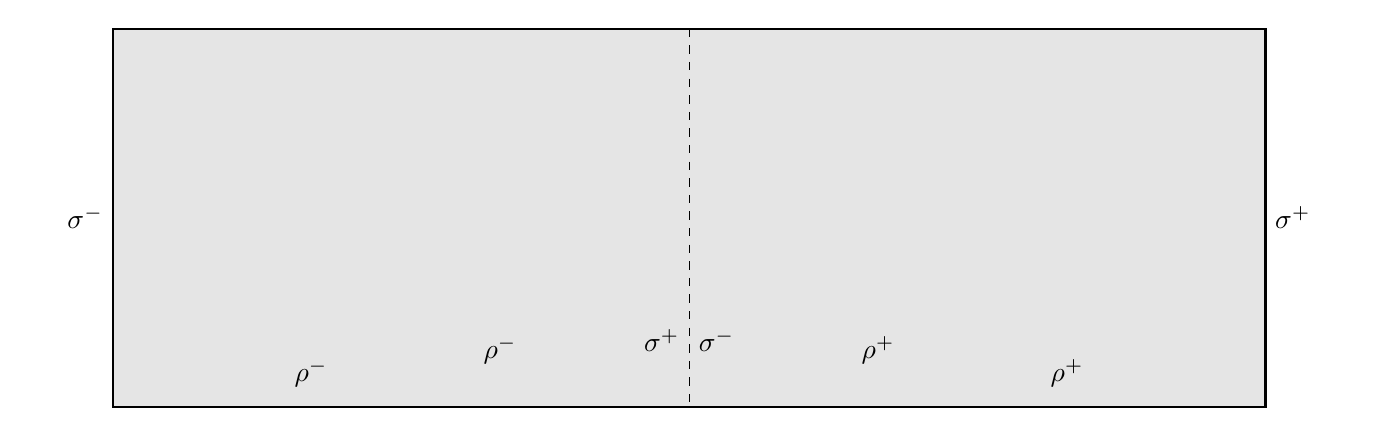
\begin{tikzpicture}[scale=1.2]
    \draw[fill=black,fill opacity=0.1,thick] (-6.1,2) rectangle (6.1,-2);

    \foreach \y in {1.25,0.75,...,-1.25}
    {
        \foreach \k in {-5,-3,...,5}
        {
            \ele{\k,\fpeval{(0.65+0.08*(abs(\k))^1.2)*\y}}{\fpeval{\y*\k*2}}
        }  
    }

    \draw[dashed] (0,2)--(0,-2);

    \clip rectangle (-7,-2) rectangle (7,2);

    \node[left]  at (-6.1,0)   {$\sigma^{-}$};
    \node[right] at (+6.1,0)   {$\sigma^{+}$};
    \node[below] at (-4,-1.4)  {$\rho^{-}$};
    \node[below] at (-2,-1.15) {$\rho^{-}$};
    \node[left]  at (0,-1.3)  {$\sigma^{+}$};
    \node[right] at (0,-1.3)  {$\sigma^{-}$};
    \node[below] at (+2,-1.15) {$\rho^{+}$};
    \node[below] at (+4,-1.4)  {$\rho^{+}$};
\end{tikzpicture}
